% Generated by thesis/ch7/exp1/networks.py -- do not edit by hand.
\ifdefined\netfigheight\else\newlength{\netfigheight}\setlength{\netfigheight}{0.9\textwidth}\fi
\begin{sidewaysfigure}
  \centering
  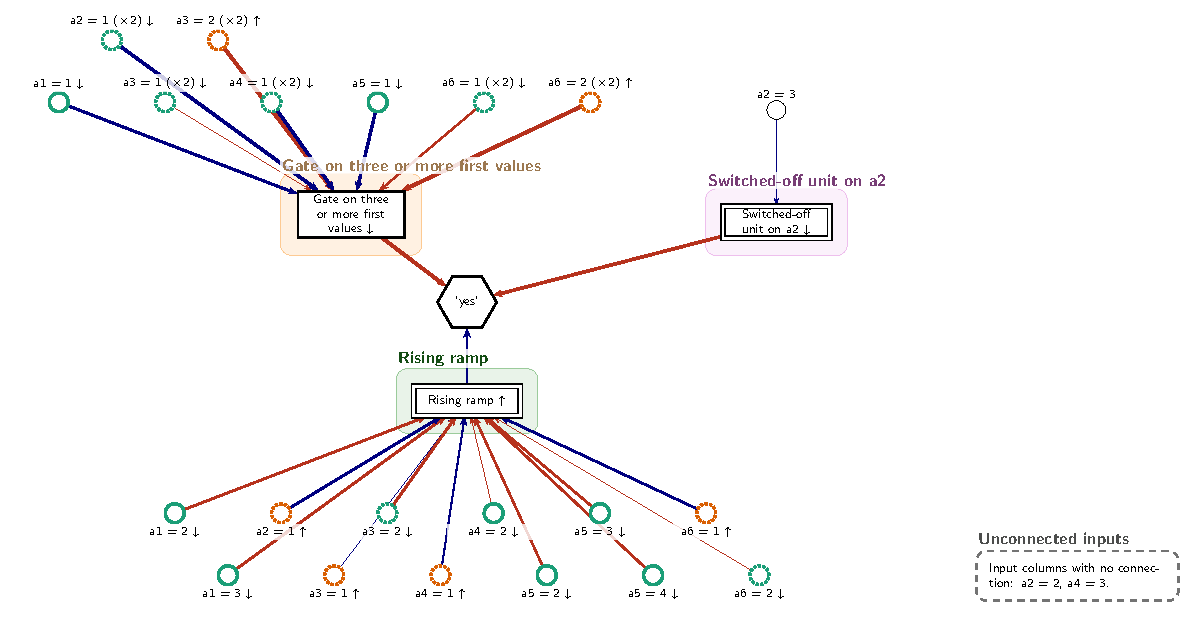
\includegraphics[width=\textheight,height=\netfigheight,keepaspectratio]{figures/exp1/networks/paper-monk2-explained}
  \caption{MONK-2, original network: the explained network, every unit nested by part. Shaded boxes: the explanation's parts (inner boxes: sub-parts); white box: a part's output (dashed: a sum standing for the output unit's addition, grey edge). Each input is drawn under every part that reads it (dotted outline, $\times n$: read by $n$ parts); a variable with many levels is drawn once, its edges labelled with their number and weight range (purple: both signs). Orange outline and up arrow: raises the final prediction; teal and down arrow: lowers it; grey and double arrow: depends. Double outline: acts at a fixed rate everywhere (dashed double: on the observed data). Edges as in Figure~\ref{fig:exp1-net-paper-monk2-raw}. Dashed grey box, right: the annotation of the input columns with no connection, outside the root.}
  \label{fig:exp1-net-paper-monk2-explained}
\end{sidewaysfigure}
